%-------------------------------------------------------------------------------
% GOVERNING EQUATIONS
%-------------------------------------------------------------------------------

\section{Governing Equations} \label{sec:gov_equ}

The following presents an overview of the physical and mathematical framework
for the 2D cavity flow problem introduced in section \ref{sec:driven_cav}. The
aim is to show the theory regarding the Navier-Stokes equations and the
stream-function formulation. \\

An incompressible Newtonian fluid in a domain $\Omega$ is governed by the
Navier-Stokes equations which are,

\begin{align}
\frac{\partial \mathbf{u}}{\partial t} + 
  \mathbf{u} \cdot \nabla \mathbf{u} &= 
  - \frac{1}{\rho} \nabla p + \mu \nabla^2 \mathbf{u} + \mathbf{g},
  \label{eq:ns3d} \\
\nabla \cdot \mathbf{u} &= 0 \label{eq:cont3d},
\end{align}

where $\mathbf{u}$ denotes the velocity vector (2D or 3D). $p$ is the pressure,
$\rho$ is the constant fluid density, $\nu$ is the kinematic viscosity and
$\mathbf{g}$ defines the body acceleration acting on the fluid. The first
equation represents the conservation of momentum, while the second is the
continuity equation. Furthermore, boundary conditions must be applied for these
equations on the domain $\Omega$. \\

For cavity flow problem in a plane, we consider the 2D form of the above
equations without body acceleration. They can be written explicitly for the two
spatial components as, 

\begin{align}
\frac{\partial u}{\partial t} + u \frac{\partial u}{\partial x} 
  + v \frac{\partial u}{\partial y} &= 
  - \frac{1}{\rho}\frac{\partial p}{\partial x}
  + \nu \left(\frac{\partial^2 u}{\partial x^2}
  + \frac{\partial^2 u}{\partial y^2}\right) \label{eq:ns2d-u}, \\
\frac{\partial v}{\partial t} + u \frac{\partial v}{\partial x}
  + v \frac{\partial v}{\partial y} &=
  - \frac{1}{\rho}\frac{\partial p}{\partial y} 
  + \nu \left(\frac{\partial^2 v}{\partial x^2}
  + \frac{\partial^2 v}{\partial y^2}\right) \label{eq:ns2d-v}, \\ 
\frac{\partial u}{\partial x}
  + \frac{\partial v}{\partial y} &= 0 \label{eq:cont2d}.
\end{align}

$u$ and $v$ denote the velocities in the $x$ and $y$ directions, respectively.
Equations \eqref{eq:ns2d-u}-\eqref{eq:cont2d} build the underlying framework
for the analysis of the 2D cavity flow. \\

In the case of a 2D incompressible fluid, it is possible to introduce a scalar
function $\Psi(x,y,t)$ called the streamfunction which is defined such that,

\begin{align}
u & = \frac{\partial \Psi}{\partial y}, \label{eq:str_defx} \\
v & = -\frac{\partial \Psi}{\partial x}. \label{eq:str_defy} 
\end{align}

By its definition, the streamfunction satisfies the continuity equation and
therefore the incompressibility condition. Regarding the momentum equations,
the expressions \eqref{eq:str_defx} and \eqref{eq:str_defy} can be used to
obtain a formulation of the Navier-Stokes that only involves the streamfunction
and where the pressure can be eliminated \citep{landau1987}:

\begin{align}
\partial_t \Delta \Psi = \nu \Delta^2 \Psi
  + (\partial_x \Psi) \partial_y(\Delta \Psi)
  - (\partial_y \Psi) \partial_x(\Delta \Psi). \label{eq:str_dim}
\end{align}

For a shorter notation, the partial derivates of the streamfunction are denoted
as subscripts in the equation above and from now on. \\

It is important to note that $\Psi = constant$ represents the family of curves
of the streamline \citep{landau1987}. Hence, if we know the streamfunction, we
can visualize the streamlines by setting the function to different constant
values.

\subsection{Nondimensionalization}

Viewing a non-dimensional version of the problem is standard to analyze the
cavity flow (figure \ref{fig:cav_4s}). The relations \eqref{eq:scl} shows the
characteristic scales of the 2D cavity. We will use the same length scale $l$
for both sides i.e. a square and thus an aspect ratio of $1$. Furthermore, as
the magnitude for our regularized boundary conditions is set to be the equal
for all lids, we can use the same velocity scale $U$.

\begin{equation}
\begin{split}
\left[ l \right] &= length  \\
\left[ U \right] &= length*time^{-1} \\
\left[ \Psi \right] &= length^2*time^{-1} \\
\left[ \frac{l}{U} \right] &= time \quad \text{(dynamic time)} \\
\end{split}
\label{eq:scl}
\end{equation}

All parameters can now be made dimensionless by defining $x = l x^*$, $y = l
y^*$, $t = \frac{l}{U} t^*$, $\Psi = lU \Psi^*$. Additionally, the
non-dimensional operators are scaled as $\partial_t = \frac{U}{l}
\partial_{t^*}$, $\partial_x = \frac{1}{l} \partial_{x^*}$, $\partial_y =
\frac{1}{l} \partial_{y^*}$ and $\Delta_* = \frac{1}{l^2} \Delta_{x^*}$. Plugin
these definitions into \eqref{eq:str}, simplifying and dividing by
$\frac{U^2}{L^2}$ we get,

\begin{align*}
\partial_{t^*} \Delta_* \Psi^* = \frac{\nu U}{l} \Delta^2_* \Psi^*
  + (\partial_x^* \Psi^*) \partial_y^*(\Delta_* \Psi^*)
  - (\partial_y^* \Psi^*) \partial_x^*(\Delta_* \Psi^*). 
\end{align*}

We notice that we can recover the Reynolds number $\Rey = \frac{Ul}{\nu}$ that,
as a non-dimensional parameter, characterizes the relative importance of
inertial forces and viscous forces in the flow. For clarity, we will omit ($*$)
notation. All quantities will correspond to the dimensionless variables. The
final equation reads,

\begin{align}
\partial_t \Delta \Psi = \frac{1}{\Rey} \Delta^2 \Psi
  + (\partial_x \Psi) \partial_y(\Delta \Psi)
  - (\partial_y \Psi) \partial_x(\Delta \Psi). \label{eq:str}
\end{align}

This equation will be the foundation for the numerical investigation later on.
The equation is non-dimensional and only depends on the scalar-valued
streamfunction and the Reynolds number. It is a nonlinear ordinary differential
equation of order 4. Different dynamics and regimes can be analyzed by changing
the Reynolds number.

\subsection{The regularized four-sided lid-driven Cavity Flow (R4CF)} \label{sec:r4sc}

Illustrated below is the domain for the four-sided cavity flow problem. In
order to differentiate between various states, we need to monitor not only the
streamfunction value at the center, but also the horizontal and vertical
velocities at the left and top midpoints of the domain. The motivation for
using this normalized domain centered at the origin instead of the classical
$[0,1]\times[0,1]$ is that, on the one hand, the reflectional symmetries of the
flow are more natural, just implying a change of sign of the spatial variables
$x$ or $y$. On the other hand, the $[-1,1]$ interval is the canonical domain
for orthogonal polynomials. 

\begin{figure}[ht]
\centering
\begin{tikzpicture}[scale=2.7]

  \draw (-1,-1) rectangle (1,1);
  \draw (-1,-1) rectangle (1,1);

  \draw[->] (-1.2,0) -- (1.2,0) node[right] {$x$};
  \foreach \x in {-1,-0.5,0.5,1}
      \draw (\x,-0.02) -- (\x,0.02) node[right=-7pt, below=4pt] {\small $\x$};
  
  \draw[->] (0,-1.2) -- (0,1.2) node[above] {$y$};
  \foreach \y in {-1,-0.5,0.5,1}
    \draw (-0.02,\y) -- (0.02,\y) node[below=5pt, left=4pt] {\small $\y$};

  \node at (0.22,0.5) {$u_T, v_T$};
  \fill (0, 0.5) circle [radius=0.6pt];

  \node at (-0.5,0.1) {$u_L, v_L$};
  \fill (-0.5,0) circle [radius=0.6pt];

  \node at (0.22,0.1) {$\Psi_{center}$};
  \fill (0,0) circle [radius=0.6pt];
\end{tikzpicture}
\caption{Square domain $(x,y) \in [-1,1]\times[-1,1]$ for the four-sided cavity.}
\label{fig:cav_domain}
\end{figure}

All lids have the same tangential velocity. The discontinuous boundary of the
four-sided problem is,

\begin{eqnarray}
u(x,\pm 1,t) & = \pm 1,\label{non_reg_u_bca} \\
v(x,\pm 1,t) & = 0, \\
u(\pm 1,y,t) & = 0, \\
v(\pm 1,y,t) & = \pm 1,,\label{non_reg_u_bcb}
\label{non_reg_u_bc}
\end{eqnarray}

To discretize \eqref{eq:str} using a spectral method, \eqref{non_reg_u_bca} and
\eqref{non_reg_u_bcb} are replaced by the regularized boundary conditions

\begin{eqnarray}
u(x,\pm 1,t) & = & \pm\left[\left(\rme^{k_0(x - 1)} - 1\right)
  \left(\rme^{-k_0(x + 1)} - 1\right)\right]^2,\label{reg_u_bca} \\
v(\pm 1,y,t) & = & \pm\left[\left(\rme^{k_0(y - 1)} - 1\right)
  \left(\rme^{-k_0(y + 1)} - 1\right)\right]^2,\label{reg_u_bcb}
\end{eqnarray}

The exponential regularization function is adapted from \citet{lopez2017}. Where
$k_0$ is a suitable parameter controlling the slope of the decay of the
velocity profile near the corners. In this study, we set $k_0=10$ to get a
suitable but not too extreme decay for the velocity at the edges. 

\begin{figure}[ht]
\center
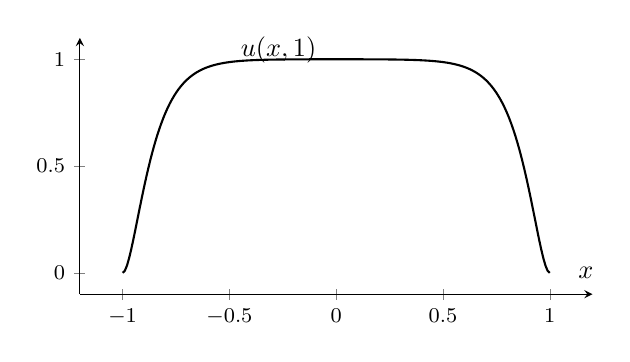
\begin{tikzpicture}[scale=0.95]
  \begin{axis}[
    xlabel={$x$},
    ylabel={$u(x, 1)$},
    xlabel style={at=(current axis.right of origin), anchor=west}, 
    ylabel style={at=(current axis.above origin), anchor=east, rotate=-90},
    domain=-1.0:1.0,
    samples=200,
    axis lines=left,
    xmin=-1.0, xmax=1.0,
    ymin=0.0, ymax=1.0,
    ticklabel style={font=\footnotesize},
    enlargelimits=true,
    axis equal image
  ]
    \addplot[black, thick] {((exp(10*(x-1))-1)*(exp(-10*(x+1))-1))^2};
  \end{axis}
\end{tikzpicture}
\caption{\label{bc_profile} Regularized horizontal velocity profile
  \eqref{reg_u_bca} at the top wall $y=1$ for $k_0=10$.}
\end{figure}

The regularized boundary conditions impose a zero velocity at all four cavity
corners. Figure \ref{bc_profile} shows such a profile for the regularization
parameter $k_0=10$.

\subsection{Scaling the Reynolds number} \label{sec:scale}

The previous literature has used a different domain, namely $[0,1] \times
[0,1]$ for the four-sided cavity flow. The reference length $l_{ref}$ used in
\citet{wahba2009} and the subsequent studies is therefor half the length $l$
used here, therefore

\begin{align}
\Rey = \frac{U \cdot l}{\nu} 
  = \frac{sU_{ref} \cdot 2l_{ref}}{\nu} = 2s \cdot \Rey_{ref}.
\end{align}

The scaling factor is $s=\frac{1}{2}$, and the Reynolds number of previous
studies has to be divided by $2$. In all further comparisons of results, the
reference Reynolds numbers of previous works will be scaled to the presented
symmetric domain.


\subsection{A physical or mathematical problem}

The final important point is that the 2D problem must be studied cautiously.
The paper of \cite{eturk2009} concludes that the single lid-driven cavity is a
fictitious flow at high Reynolds numbers. Fictitious meaning that the problem
from a physical point of view would no longer be two-dimensional. However,
numerical solutions exist at high Reynolds numbers for the 2D case. 

Additionally, it is hard to replicate the lid-driven cavity experimentally with
regularized boundary conditions. This problem is even worse considering the
four-sided cavity flow version and different velocity directions at the lid.

Using a regularized version, as presented above, will help for numerically
accurate results, but additionally is even harder to reproduce in practice.
From the point of view of a benchmark for an instability analysis for different
solvers, the resulting flow (if fictional or not) should at least be accurately
computable. That being said, this report will focus on the main aspect, which
is the accurate computation of a well-posed mathematical problem. 
